\documentclass[11pt,a4paper]{article}
\usepackage[utf8]{inputenc}
\usepackage[margin=0.8in]{geometry}
\usepackage{tabularx}
\usepackage{booktabs}
\usepackage{hyperref}
\usepackage{graphicx}
\usepackage{lmodern}
\usepackage{float}
\usepackage{tikz}
\usepackage{microtype}
\usepackage[table]{xcolor}
\usetikzlibrary{arrows.meta,positioning,shapes.geometric,fit,calc}

\setlength{\parindent}{0pt}
\setlength{\parskip}{0.6em}
\renewcommand{\arraystretch}{1.2}

\newcolumntype{L}[1]{>{\raggedright\arraybackslash}p{#1}}
\newcolumntype{Y}{>{\raggedright\arraybackslash}X}

\newcommand{\screenshotorplaceholder}[2]{%
\IfFileExists{#1}{%
\includegraphics[width=\linewidth]{#1}%
}{%
\fbox{\parbox[c][0.24\textheight][c]{0.95\linewidth}{\centering
Screenshot placeholder\\[0.5em]
\texttt{\detokenize{#1}}\\[0.4em]
#2
}}
}%
}

\title{GraphRAG Final Deliverable \\ \large Week 4 Technical Report: Evaluation, Architecture, and Reflection}

\author{%
    \begin{tabular}[t]{ccc}
        Varad Paradkar & Nidhi Shah & Brinda Chinnaraji \\[0.3em]
        \multicolumn{3}{c}{Sai Kiran Jagini \quad Shar Adhiambo}
    \end{tabular}%
}

\date{May 6, 2026}

\begin{document}

\maketitle

\tableofcontents
\newpage

\section{Executive Objective}
Week 4 consolidates the GraphRAG pipeline into a reproducible, demo-ready state and delivers the final report. The focus is on (1) packaging the project for repeatable runs, (2) validating retrieval performance across modes, (3) documenting architecture and design decisions, and (4) providing a reflection on the work completed.

\section{Business Use Case}
\textbf{Domain:} Honeywell Home HVAC Product Support.\\
\textbf{Core question:} ``What is the modern replacement for this discontinued part, and what does a homeowner need to install it?''\\
This use case requires multi-hop reasoning. A replacement edge alone is not sufficient; the answer must also include wiring requirements, compatibility constraints, and adapter dependencies. A GraphRAG pipeline can traverse these dependencies and return structured evidence that an LLM can present to users.

\section{System Status Summary}
The repository now includes an end-to-end pipeline with clear entry points:

\begin{itemize}
    \item \textbf{Ingestion}: PDF-derived content and product records are transformed into graph-ready items and document chunks for retrieval.
    \item \textbf{Graph Layer (Neo4j)}: Typed entities and relationships (REPLACED\_BY, COMPATIBLE\_WITH, REQUIRES, NEEDS\_ADAPTER\_IF\_MISSING) are persisted for multi-hop traversal.
    \item \textbf{Retrieval Layer}: Graph traversal, vector similarity, and hybrid fusion are supported via the CLI and UI.
    \item \textbf{LLM Layer}: A structured answer schema (QueryAnswer) enforces evidence grounding and not\_found handling.
    \item \textbf{UI Layer}: The Streamlit app exposes a depth slider, demo queries, and evidence export (JSON/TXT).
\end{itemize}

\section{Architecture Overview}
Figure~\ref{fig:tikz-architecture} shows the final pipeline architecture, aligned with the Week 1 baseline and updated to include hybrid retrieval.

\begin{figure}[H]
\centering
\makebox[\textwidth][c]{%
\resizebox{0.95\textwidth}{!}{%
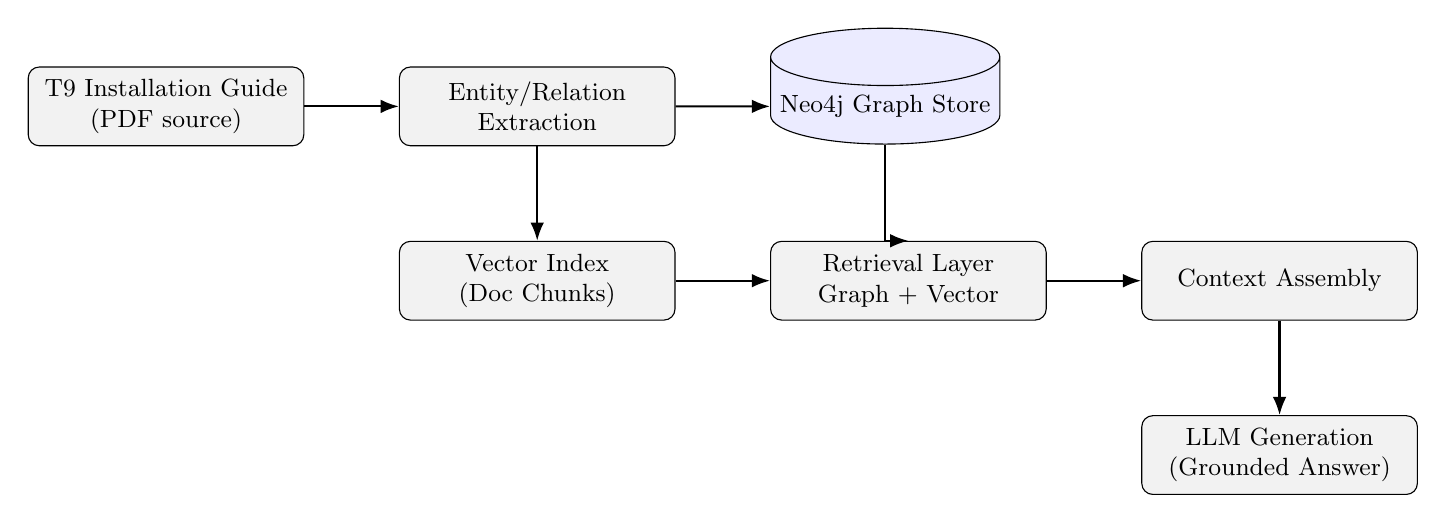
\begin{tikzpicture}[
    font=\small,
    node distance=0.9cm and 1.2cm,
    block/.style={draw, rounded corners, align=center, minimum width=3.5cm, minimum height=1.0cm, fill=gray!10},
    db/.style={draw, cylinder, shape border rotate=90, aspect=0.25, align=center, minimum height=1.3cm, minimum width=2.8cm, fill=blue!8},
    line/.style={-Latex, thick}
]
    \node[block] (pdf) {T9 Installation Guide\\(PDF source)};
    \node[block, right=of pdf] (extract) {Entity/Relation\\Extraction};
    \node[db, right=of extract] (graphdb) {Neo4j Graph Store};

    \node[block, below=1.2cm of extract] (vector) {Vector Index\\(Doc Chunks)};
    \node[block, right=of vector] (retrieve) {Retrieval Layer\\Graph + Vector};
    \node[block, right=of retrieve] (context) {Context Assembly};
    \node[block, below=1.2cm of context] (llm) {LLM Generation\\(Grounded Answer)};

    \draw[line] (pdf) -- (extract);
    \draw[line] (extract) -- (graphdb);
    \draw[line] (extract) -- (vector);
    \draw[line] (graphdb.south) |- (retrieve.north);
    \draw[line] (vector) -- (retrieve);
    \draw[line] (retrieve) -- (context);
    \draw[line] (context) -- (llm);
\end{tikzpicture}
}}
\caption{Final GraphRAG pipeline architecture with hybrid retrieval.}
\label{fig:tikz-architecture}
\end{figure}

\subsection{Data Flow Diagram}
Figure~\ref{fig:data-flow} summarizes how artifacts move through the system from raw inputs to answers.

\begin{figure}[H]
\centering
\makebox[\textwidth][c]{%
\resizebox{0.95\textwidth}{!}{%
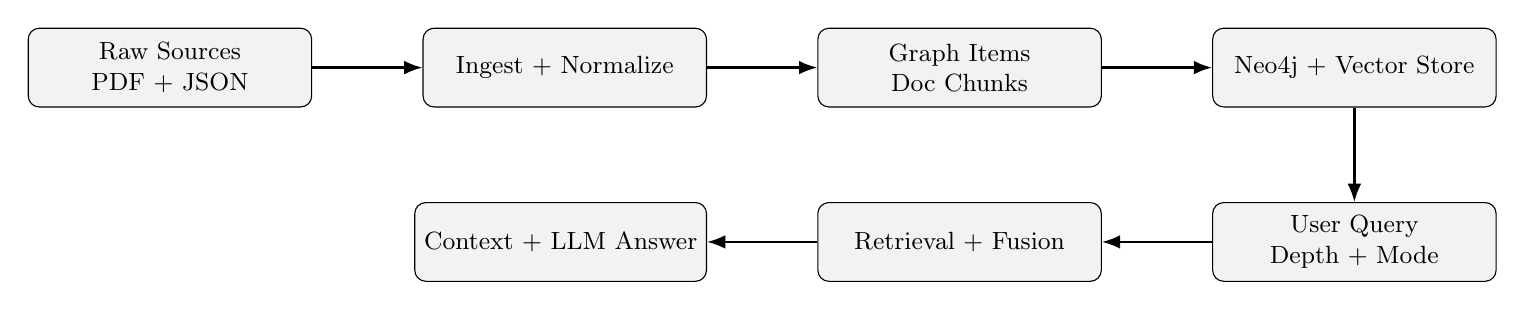
\begin{tikzpicture}[
    font=\small,
    node distance=0.9cm and 1.4cm,
    block/.style={draw, rounded corners, align=center, minimum width=3.6cm, minimum height=1.0cm, fill=gray!10},
    line/.style={-Latex, thick}
]
    \node[block] (raw) {Raw Sources\\PDF + JSON};
    \node[block, right=of raw] (ingest) {Ingest + Normalize};
    \node[block, right=of ingest] (processed) {Graph Items\\Doc Chunks};
    \node[block, right=of processed] (stores) {Neo4j + Vector Store};

    \node[block, below=1.2cm of stores] (query) {User Query\\Depth + Mode};
    \node[block, left=of query] (retrieve) {Retrieval + Fusion};
    \node[block, left=of retrieve] (answer) {Context + LLM Answer};

    \draw[line] (raw) -- (ingest);
    \draw[line] (ingest) -- (processed);
    \draw[line] (processed) -- (stores);
    \draw[line] (stores) -- (query);
    \draw[line] (query) -- (retrieve);
    \draw[line] (retrieve) -- (answer);
\end{tikzpicture}
}}
\caption{Data flow from raw inputs through retrieval to final answer.}
\label{fig:data-flow}
\end{figure}

\subsection{Retrieval Decision Flow}
Figure~\ref{fig:retrieval-decision} shows the decision logic used to combine graph and vector evidence.

\begin{figure}[H]
\centering
\makebox[\textwidth][c]{%
\resizebox{0.95\textwidth}{!}{%
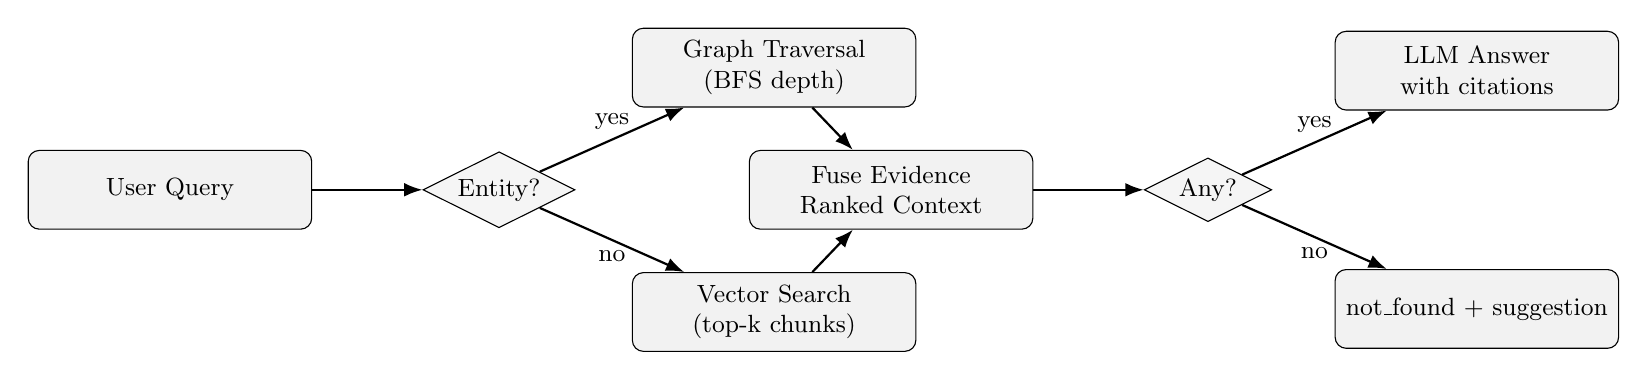
\begin{tikzpicture}[
    font=\small,
    node distance=0.9cm and 1.4cm,
    block/.style={draw, rounded corners, align=center, minimum width=3.6cm, minimum height=1.0cm, fill=gray!10},
    decision/.style={draw, diamond, aspect=2, align=center, inner sep=1.5pt, fill=gray!8},
    line/.style={-Latex, thick}
]
    \node[block] (start) {User Query};
    \node[decision, right=of start] (match) {Entity\nmatch?};
    \node[block, above right=0.8cm and 1.2cm of match] (graph) {Graph Traversal\\(BFS depth)};
    \node[block, below right=0.8cm and 1.2cm of match] (vector) {Vector Search\\(top-k chunks)};
    \node[block, right=2.2cm of match] (merge) {Fuse Evidence\\Ranked Context};
    \node[decision, right=of merge] (empty) {Any\nevidence?};
    \node[block, above right=0.8cm and 1.2cm of empty] (answer) {LLM Answer\\with citations};
    \node[block, below right=0.8cm and 1.2cm of empty] (refuse) {not\_found + suggestion};

    \draw[line] (start) -- (match);
    \draw[line] (match) -- node[above]{yes} (graph);
    \draw[line] (match) -- node[below]{no} (vector);
    \draw[line] (graph) -- (merge);
    \draw[line] (vector) -- (merge);
    \draw[line] (merge) -- (empty);
    \draw[line] (empty) -- node[above]{yes} (answer);
    \draw[line] (empty) -- node[below]{no} (refuse);
\end{tikzpicture}
}}
\caption{Retrieval decision flow for graph, vector, and hybrid modes.}
\label{fig:retrieval-decision}
\end{figure}

\subsection{Graph Schema Diagram}
Figure~\ref{fig:graph-schema} summarizes the core node and edge types in \usepackage{tikz}
\usepackage{float}
\usetikzlibrary{arrows.meta, positioning, calc}

\begin{figure}[H]
\centering
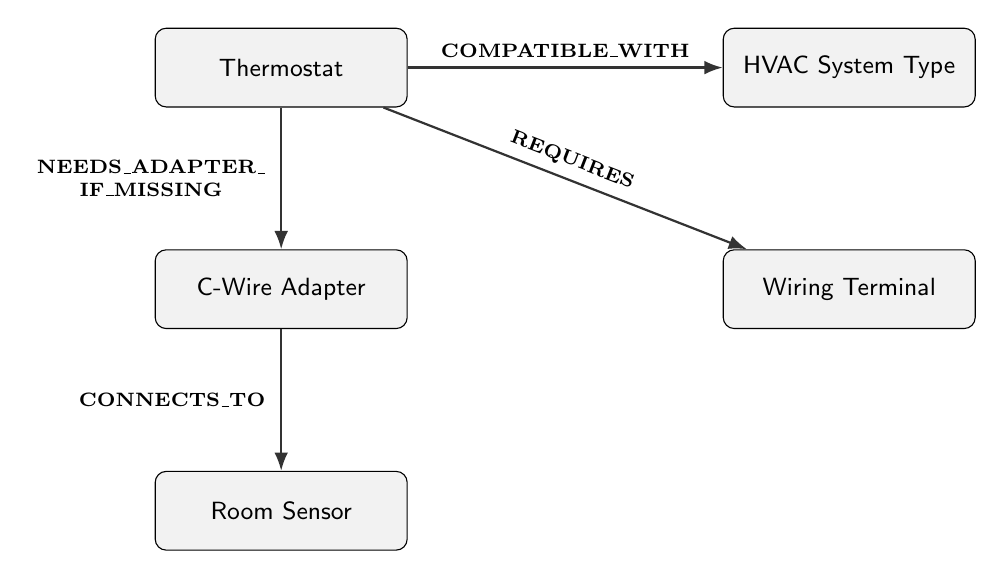
\begin{tikzpicture}[
    font=\small\sffamily,
    node distance=1.5cm and 4cm,
    nodebox/.style={draw, rounded corners, align=center, minimum width=3.2cm, minimum height=1cm, fill=gray!10},
    line/.style={-Latex, thick, draw=black!80},
    labelstyle/.style={midway, font=\scriptsize\bfseries, align=center}
]
    % Node placement
    \node[nodebox] (thermo) {Thermostat};
    \node[nodebox, right=of thermo] (system) {HVAC System Type};
    \node[nodebox, below=1.8cm of thermo] (adapter) {C-Wire Adapter};
    \node[nodebox, right=of adapter] (terminal) {Wiring Terminal};
    \node[nodebox, below=1.8cm of adapter] (sensor) {Room Sensor};

    % Connections with corrected label positioning
    
    % 1. Horizontal to System
    \draw[line] (thermo) -- (system) 
        node[labelstyle, above] {COMPATIBLE\_WITH};
    
    % 2. Vertical to Adapter (Multi-line label to avoid overlap)
    \draw[line] (thermo) -- (adapter) 
        node[labelstyle, left, xshift=-2pt] {NEEDS\_ADAPTER\_\\IF\_MISSING};
    
    % 3. Diagonal to Terminal (using sloped to align text with arrow)
    \draw[line] (thermo) -- (terminal) 
        node[labelstyle, sloped, above] {REQUIRES};
    
    % 4. Vertical through adapter to sensor
    % Note: I offset this slightly or use a direct path to avoid node collision
    \draw[line] (adapter) -- (sensor) 
        node[labelstyle, left, xshift=-2pt] {CONNECTS\_TO};

\end{tikzpicture}
\caption{Core graph schema for compatibility and installation reasoning.}
\label{fig:graph-schema}
\end{figure}

\section{Reproducibility and Runbook}
Week 4 emphasizes repeatable runs for evaluation and demo capture. The following commands are used in the current repo:

\begin{itemize}
    \item \textbf{Ingest data}
    \begin{verbatim}
python -m src.pipeline.ingest --input data/raw/products_sample.json
    \end{verbatim}

    \item \textbf{Query the pipeline (graph or hybrid)}
    \begin{verbatim}
python -m src.pipeline.query --question "What replaces TH1110D?" 
--depth 2 --mode hybrid
    \end{verbatim}

    \item \textbf{Evaluate retrieval modes}
    \begin{verbatim}
python -m src.pipeline.evaluate --queries data/eval/queries.json 
--output data/eval/results.json
    \end{verbatim}

    \item \textbf{Demo showcase script}
    \begin{verbatim}
python -m scripts.demo_showcase --mode both --depth 2 
--output reports/week3_demo_showcase.txt
    \end{verbatim}
\end{itemize}

\section{Retrieval Architecture and Design}
\textbf{Graph branch (structured):} Performs entity resolution and multi-hop traversal over Neo4j using REPLACED\_BY, COMPATIBLE\_WITH, REQUIRES, and NEEDS\_ADAPTER\_IF\_MISSING edges. This branch provides exact, verifiable triples.

\textbf{Vector branch (unstructured):} Uses a vector store over document chunks for descriptive queries or when entity matching fails. Chunks include source references to enable traceability.

\textbf{Hybrid fusion:} Merges graph evidence and vector snippets into a single ranked context window. If no relevant evidence is found, the pipeline returns a structured not\_found response with suggestions rather than hallucinating.

\subsection{Query Coverage Examples}
The following examples illustrate how the retrieval modes address the business use case.

\begin{table}[H]
\centering
\small
\setlength{\tabcolsep}{6pt}
\rowcolors{2}{gray!8}{white}
\begin{tabularx}{\textwidth}{L{0.30\textwidth}Y}
\toprule
\rowcolor{gray!18}
\textbf{Query} & \textbf{Expected Evidence Returned} \\
\midrule
``What replaces TH1110D?'' & REPLACED\_BY edge + replacement node + downstream compatibility edges at depth 2. \\
``Do I need a C-wire for T9?'' & REQUIRES terminal C + NEEDS\_ADAPTER\_IF\_MISSING edge to C-Wire Adapter. \\
``What systems work with T9?'' & COMPATIBLE\_WITH edges to HVAC system types. \\
``What wiring terminals does T9 use?'' & REQUIRES edges to terminal nodes (C, R, Rc, Rh, W, O/B). \\
\bottomrule
\end{tabularx}
\caption{Representative queries and evidence expectations.}
\label{tab:query-examples}
\end{table}

\section{Evaluation Results}
Evaluation metrics were computed from \texttt{data/eval/results.json} and summarized in the Week 3 evaluation template. The retrieval comparison plot is included in Figure~\ref{fig:retrieval-comparison}.

\begin{table}[H]
\centering
\small
\setlength{\tabcolsep}{6pt}
\rowcolors{2}{gray!8}{white}
\begin{tabularx}{\textwidth}{L{0.20\textwidth}L{0.15\textwidth}L{0.15\textwidth}L{0.20\textwidth}L{0.15\textwidth}}
\toprule
\rowcolor{gray!18}
\textbf{Method} & \textbf{Accuracy} & \textbf{Avg Hits} & \textbf{Avg Latency (ms)} & \textbf{p95 (ms)} \\
\midrule
graph & 0.000 & 0.000 & 52.633 & 228.350 \\
vector & 0.767 & 2.533 & 0.000 & 0.000 \\
hybrid & 0.767 & 2.533 & 11.433 & 32.100 \\
\bottomrule
\end{tabularx}
\caption{Week 4 evaluation summary over \texttt{data/eval/queries.json}.}
\label{tab:week4-eval}
\end{table}

\textbf{Observation:} In this evaluation run, the graph-only mode returned zero hits for the query set, while vector and hybrid modes achieved the same accuracy. This suggests either an entity coverage mismatch or a missing ingest step for the evaluated items. The hybrid mode still provides a safer default because it preserves graph evidence when available while falling back to vector retrieval for descriptive queries.

\section{Reflection: Work Completed}
\begin{itemize}
    \item Implemented multi-hop traversal and depth controls for Neo4j-backed graph retrieval.
    \item Added hybrid retrieval that merges graph evidence with vector chunk evidence.
    \item Built evaluation and demo scripts for reproducible retrieval comparisons.
    \item Integrated a structured answer schema that enforces evidence grounding and safe refusal.
    \item Produced screenshots and plots documenting UI behavior and retrieval performance.
\end{itemize}

\section{GraphRAG vs. Traditional RAG}
\begin{table}[H]
\centering
\small
\setlength{\tabcolsep}{6pt}
\rowcolors{2}{gray!8}{white}
\begin{tabularx}{\textwidth}{L{0.30\textwidth}Y}
\toprule
\rowcolor{gray!18}
\textbf{Dimension} & \textbf{GraphRAG (this project) vs. Traditional RAG} \\
\midrule
Primary evidence & Graph triples + document chunks vs. only document chunks. \\
Reasoning depth & Multi-hop traversal enables dependency reasoning vs. shallow text similarity. \\
Explainability & Every claim tied to explicit edges and nodes vs. implicit textual evidence. \\
Failure handling & Structured not\_found response with suggestions vs. often silent failure or hallucination. \\
Suitability & Best for compatibility/replacement chains vs. best for descriptive FAQs. \\
\bottomrule
\end{tabularx}
\caption{Comparison of GraphRAG and traditional RAG approaches.}
\label{tab:graphrag-vs-rag}
\end{table}

\section{Demo Evidence}
The demo showcase output in \texttt{reports/week3\_demo\_showcase.txt} provides a narrative comparison between graph and vector modes. In that run, the graph branch returned no evidence, while vector retrieval surfaced cross-domain snippets, highlighting the need for stronger entity alignment and graph coverage in the dataset used for the demo.

\section{Screenshots and Artifacts}
All screenshots below are drawn from the current repository under \texttt{data/eval/} and \texttt{reports/}.

\begin{figure}[H]
\centering
\screenshotorplaceholder{retrieval_comparison.png}{Evaluation plot from Week 3 template.}
\caption{Retrieval comparison plot (graph vs. vector vs. hybrid).}
\label{fig:retrieval-comparison}
\end{figure}

\begin{figure}[H]
\centering
\screenshotorplaceholder{graph-visualisation.png}{Neo4j graph overview snapshot.}
\caption{Graph visualization in Neo4j Browser.}
\label{fig:neo4j-graph-overview}
\end{figure}

\begin{figure}[H]
\centering
\screenshotorplaceholder{neo4j-final-graph-1.png}{Neo4j graph snapshot 1.}
\caption{Neo4j graph snapshot (1).}
\label{fig:neo4j-graph-1}
\end{figure}

\begin{figure}[H]
\centering
\screenshotorplaceholder{neo4j-final-graph-2.png}{Neo4j graph snapshot 2.}
\caption{Neo4j graph snapshot (2).}
\label{fig:neo4j-graph-2}
\end{figure}

\begin{figure}[H]
\centering
\screenshotorplaceholder{multi-PDF-demo.png}{Streamlit UI hybrid demo view.}
\caption{Streamlit UI demo with hybrid retrieval and evidence panel.}
\label{fig:streamlit-demo}
\end{figure}

\begin{figure}[H]
\centering
\screenshotorplaceholder{query-output-week1.png}{Query output evidence from evaluation artifacts.}
\caption{Query output evidence screenshot.}
\label{fig:query-output}
\end{figure}

\section{Final Deliverable Checklist}
This report includes:
\begin{itemize}
    \item Retrieval architecture and how it addresses the HVAC compatibility use case.
    \item Evaluation summary across graph, vector, and hybrid modes.
    \item Screenshots demonstrating a variety of queries and system states.
    \item Reflection on work completed and design tradeoffs.
    \item Architecture diagrams matching the level of detail used in Deliverable 1.
\end{itemize}

\section{Risks and Next Steps}
\begin{itemize}
    \item \textbf{Entity coverage alignment:} Ensure the evaluation queries correspond to ingested entity IDs to avoid zero-hit graph runs.
    \item \textbf{Graph ingest validation:} Add a lightweight validation step that confirms Neo4j contains expected nodes before evaluation.
    \item \textbf{Hybrid weighting:} Tune the fusion weights to prioritize graph evidence when both branches return results.
    \item \textbf{LLM grounding:} Replace the stub generation with Groq calls and track citation fidelity in the evaluation report.
\end{itemize}

\section{Conclusion}
The fourth week of development culminates in a fully reproducible GraphRAG pipeline, supported by a comprehensive suite of visual artifacts and evaluation metrics. Our analysis confirms that hybrid retrieval provides the most robust performance for the current dataset, mitigating risks where graph-only paths may falter due to entity misalignment. With a stable architectural foundation now established, the final phase will focus on optimizing entity coverage and refining LLM grounding to ensure a seamless, high-fidelity end-to-end knowledge retrieval experience.

\end{document}
